\lecdate{26.06.2017}
\section{Formeln und Begriffe}
%\\
$$\text{Notation: } \PP(A,B)=\PP(A \cap B)$$
$$\PP(\bullet | A ) = \cA[0,1]$$
$$\PP(B|A)=\frac{\PP(A \cap B)}{\PP(A)} \quad \text{bzw. } \PP(B|A)\cdot \PP(A) = \PP(A,B)$$
Dies gilt nur, wenn $B$ nur von $A$ abhängig ist und nicht von weiteren. Sonst: Marginalisierung / disjunkte Zerlegung:
$$\PP(A) = \PP(A\cap (B \cup \overline{B}))=\PP((A \cap B) \cup (A \cap \overline{B}))=\PP(A \cap B) + \PP(A\cap \overline{B})=\PP(A,B)+\PP(A, \overline{B})$$
$$A, \;B \text{ unabhängig}\Leftrightarrow \PP(A \cap B)=\PP(A) \cdot \PP(B)$$
$$P\left(\sum A_k\right) = \sum \PP(A_k)$$
$$P\left(\bigcup A_k\right) \leq \sum \PP(A_k)$$
Ereignisse $A$, $B$ heißen \emph{bedingt unabhängig} gegeben $C$, wenn gilt $\PP(A,B|C) = \PP(A|C) \cdot \PP(B|C)$. Dies ist gleichwertig damit, dass $A$, $B$ unabhängig bezüglich des W-Maßes $\PP(\bullet|C)$ sind.\\
Hinweis zur Berechnung von Wahrscheinlichkeiten:
\begin{center}
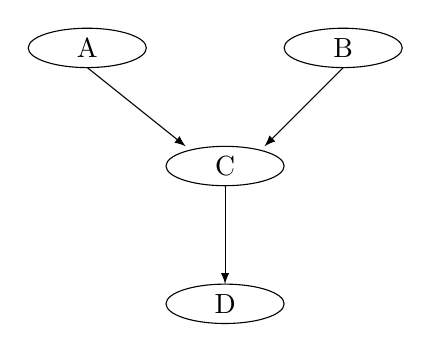
\begin{tikzpicture}[scale=.5]
\draw  (-3,1) node{C} ellipse(1.5 and 0.5);
\draw  (-3,-2.5) node{D} ellipse(1.5 and 0.5);
\draw  (-6.5,4) node{A} ellipse (1.5 and 0.5);
\draw  (0,4) node{B} ellipse (1.5 and 0.5);
\draw [-latex] (-6.5,3.5) -- (-4,1.5);
\draw [-latex](0,3.5) -- (-2,1.5);
\draw [-latex](-3,0.5) -- (-3,-2);
\end{tikzpicture}
\end{center}
$$\PP(D) = \PP(D,A,B,C) + \ldots + \PP(D, \overline{A}, \overline{B}, \overline{C})$$
$$\PP(D,A,B,C) = \PP(D|C) \cdot \PP(C|A \cap B) \cdot \PP(A) \cdot \PP(B)$$
\section{Grundlagen}

\paragraph{Beispiel} Bob hat in seinem Haus eine Alarmanlage installiert. Seine Nachbarn John und Marry rufen ihn im Büro an, wenn sie Alarm hören. Bob modelliert deren Zuverlässigkeit durch 
$$\PP(J \; | \; Al) =0,9 \qquad \PP(M \; | \; Al) =0,7$$
$$\PP(J \; | \; \overline{Al}) = 0,05 \qquad \PP(M \; | \; \overline{Al}) = 0,01$$
Sowohl ein Einbruch als auch ein Erdbeben können einen Alarm auslösen:
$$\PP(Al \; | \; Ein, \; Erd) = 0,95 \qquad \PP(Al \; |\; Ein,\; \overline{Erd}) = 0,94$$
$$\PP(Al \; | \; \overline{Ein},\; Erd) = 0,29 \qquad \PP(Al \; | \; \overline{Ein}, \; \overline{Erd}) =0,001$$
Ferner sei $\PP(Ein) = 0,001$, $\PP(Erd) = 0,002$.\\
Die Ereignisse $Erd$, $Ein$ seien unabhängig.\\
Graphisch Darstellung als Bayes'sches Netz:
\begin{itemize}
\item Knoten: Ereignisse
\item Kanten: Bedingte W'keiten
\end{itemize}
\begin{center}
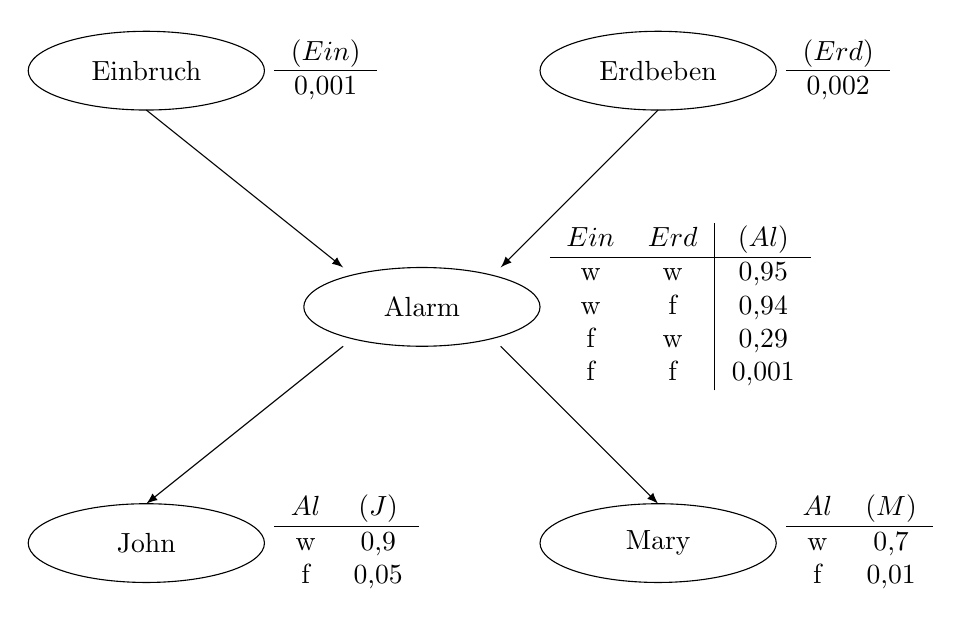
\begin{tikzpicture}
\draw  (-3,1) node{Alarm} ellipse(1.5 and 0.5);
\draw  (-6.5,4) node{Einbruch} ellipse (1.5 and 0.5);
\draw  (0,4) node{Erdbeben} ellipse (1.5 and 0.5);
\draw  (-6.5,-2) node{John} ellipse (1.5 and 0.5);
\draw  (0,-2) node{Mary} ellipse (1.5 and 0.5);
\node [right] at (-5,4) {\begin{tabular}{c}
$\PP(Ein)$\\\hline
0,001\\
\end{tabular}};
\node [right] at (1.5,4) {\begin{tabular}{c}
$\PP(Erd)$\\\hline
0,002
\end{tabular}};
\node [right] at (-5,-2) {\begin{tabular}{c c}
$Al$ & $\PP(J)$\\\hline
w & 0,9\\
f & 0,05\\
\end{tabular}};
\node [right] at (1.5,-2) {\begin{tabular}{c c}
$Al$ & $\PP(M)$\\\hline
w & 0,7\\
f & 0,01
\end{tabular}};
\node [right]at (-1.5,1) {\begin{tabular}{c c | c}
$Ein$ & $Erd$ & $\PP(Al)$\\\hline
w & w & 0,95\\
w & f & 0,94\\
f & w & 0,29\\
f & f & 0,001
\end{tabular}};
\draw [-latex] (-6.5,3.5) -- (-4,1.5);
\draw [-latex](0,3.5) -- (-2,1.5);
\draw [-latex](-4,0.5) -- (-6.5,-1.5);
\draw [-latex](-2,0.5) -- (0,-1.5);
\end{tikzpicture}
\end{center}
Wen John und Mary unabhängig auf einen Alarm reagieren, dann sind die Ereignisse $J$, $M$ unabhängig gegeben $Al$.

\section{Semantik von Bayes-Netzen}
Kanten beschreiben (bedingte) Unabhängigkeiten von Ereignissen:
\begin{center}
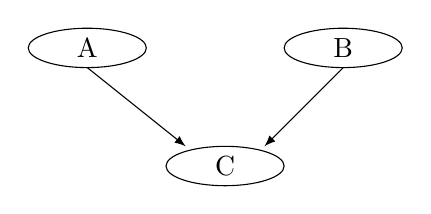
\begin{tikzpicture}[scale=.5]
\draw  (-3,1) node{C} ellipse(1.5 and 0.5);
\draw  (-6.5,4) node{A} ellipse (1.5 and 0.5);
\draw  (0,4) node{B} ellipse (1.5 and 0.5);
\draw [-latex] (-6.5,3.5) -- (-4,1.5);
\draw [-latex](0,3.5) -- (-2,1.5);
\end{tikzpicture}\\
$\to$ $A$, $B$ sind unabhängig.
\end{center}
\begin{center}
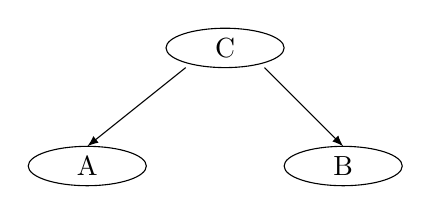
\begin{tikzpicture}[scale=.5]
\draw  (-3,1) node{C} ellipse(1.5 and 0.5);
\draw  (-6.5,-2) node{A} ellipse (1.5 and 0.5);
\draw  (0,-2) node{B} ellipse (1.5 and 0.5);
\draw [-latex](-4,0.5) -- (-6.5,-1.5);
\draw [-latex](-2,0.5) -- (0,-1.5);
\end{tikzpicture}\\
$\to$ $A$, $B$ sind unabhängig gegeben $C$.
\end{center}
Ein Bayes-Netz muss ein DAG (directed asymmetric graph) sein (enthält also keinen Loop). Dann können die Knoten topologisch sortiert werden. Dann gilt:
$$\PP(A_n|A_1, \dots, A_{n-1}=\PP(A_n|\; \mathrm{Eltern}(A_n)$$
\begin{center}
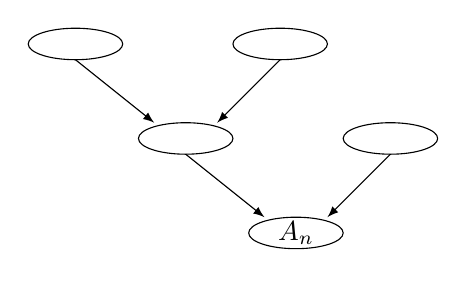
\begin{tikzpicture}[scale=.4]
\draw  (-10,7) ellipse (1.5 and 0.5);
\draw  (-3.5,7) ellipse (1.5 and 0.5);
\draw [-latex] (-10,6.5) -- (-7.5,4.5);
\draw [-latex](-3.5,6.5) -- (-5.5,4.5);
\draw  (-3,1) node{$A_n$} ellipse(1.5 and 0.5);
\draw  (-6.5,4) ellipse (1.5 and 0.5);
\draw  (0,4) ellipse (1.5 and 0.5);
\draw [-latex] (-6.5,3.5) -- (-4,1.5);
\draw [-latex](0,3.5) -- (-2,1.5);
\end{tikzpicture}
\end{center}
Daraus folgt:
\begin{align*}
\PP(A_1, \dots, A_n)&=\PP(A_n|A_1,\dots,A_{n-1})\cdot \PP(A_1, \dots, A_{n-1})\\
&= \PP(A_n|\;\mathrm{Eltern}(A_n)) \cdot \PP(A_1, \dots, A_{n-1})\\
&=\ldots \\
&= \prod_{k=1}^n \PP(A_k |\; \mathrm{Eltern}(A_k))
\end{align*}
Dabei ist $\PP(A_k|\; \mathrm{Eltern}(A_k)):=\PP(A_k)$, wenn $A_k$ keine Eltern besitzt.
\paragraph{Beispiel} 
\begin{align*}
\PP(J, Al, Ein, Erd) &= \PP(J|Al) \cdot \PP(Al|Ein, Erd) \cdot \PP(Ein) \cdot \PP(Erd)\\
&= 0,00000171
\end{align*}
\begin{align*}
\PP(J, Ein) &= \PP(J, Al, Ein, Erd) + \PP(J, \overline{Al}, Ein, Erd)\\
& \qquad +\PP(J, Al, \overline{Erd}, Ein) + \PP(J, \overline{Al}, Ein, \overline{Erd})\\
&= \ldots = 0,000849
\end{align*}
Entsprechend ergibt sich $\PP(J) = 0,052$.\\
$\PP(Ein|J) = \frac{\PP(Ein, J)}{\PP(J)}=0,016$. Diese Zahl ist so gering, da die WK für den Einbruch sehr gering ist.

\section{Komplexität der Inferenz in Bayes'schen Netzen}
\lecdate{03.07.2017}
Die exakte Inferenz (Berechnung von W'keiten) ist NP-vollständig. D.h., es ist kein effizienter (polynomieller) Algorithmus zur Berechnung der W'keiten bekannt.

Bei einem Bayes'schen Netz mit den Knoten $A_1, \dots, A_n$ muss $\PP(A_n)$ im Allgemeinen durch eine disjunkte Zerlegung folgender Form sein:
$$\PP(A_n) = \PP(A_n, A_1, \dots, A_{n-1})+\ldots + \PP(A_n, \overline{A}_1, \dots,  \overline{A}_{n-1})$$
Diese Summe besteht aus $2^{n-1}$ Summanden. Der Aufwand zur Berechnung von $\PP(A_n)$ wächst daher exponentiell in $n$.
$$SAT=\{F\;|\; F \text{ ist eine erfüllbare Formel der Aussagenlogik}\}$$
$SAT$ ist NP-vollständig. Man kann zeigen: Aus einem effizienten Algorithmus für Bays'sche Netze ließe sich ein effizienter Entscheidungsalgorithmus für $SAT$ konstruieren.

\paragraph{Beispiel} Sei $F=(A \vee B \vee C) \wedge (A \vee \neg B) \wedge \neg C$\\
(Vorgehen: Eingangsknoten auf $\frac{1}{2}$ setzen, prüfen, ob Ergebnis erfüllbar ist)\\
Daraus konstruieren wir folgendes Bays'sches Netz:
\begin{center}
{
\renewcommand{\arraystretch}{1}
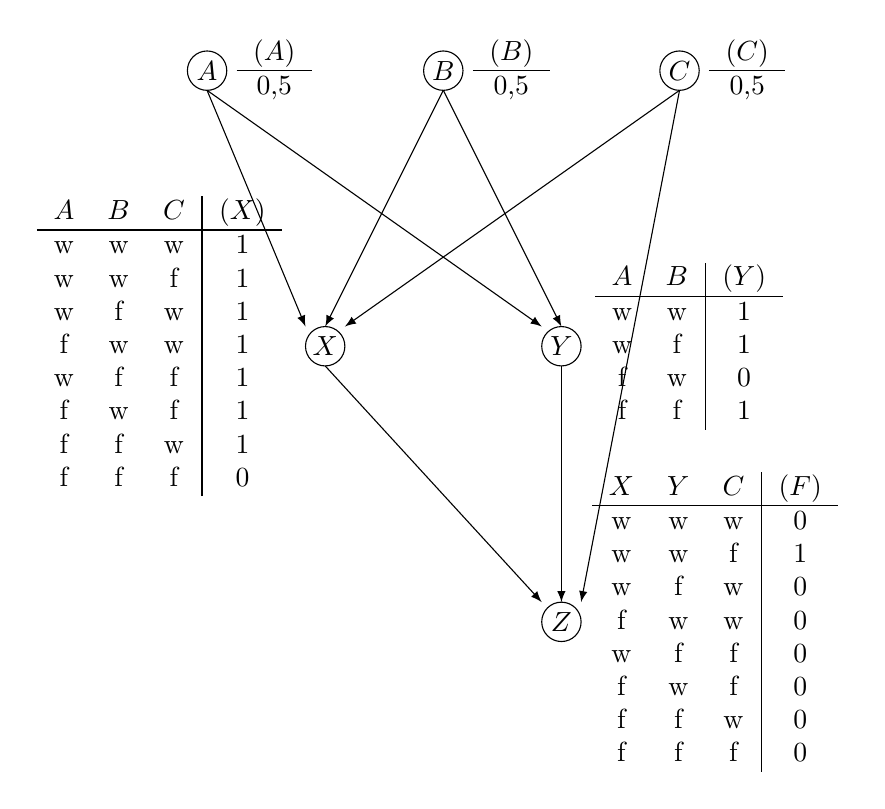
\begin{tikzpicture}[scale=.5]
\draw  (-6,0) node{$A$} ellipse (0.5 and 0.5);
\node [right, align=left] at (-5.5,0) {
\begin{tabular}{c}
$\PP(A)$\\\hline
0,5\\
\end{tabular}
};
\draw  (0,0) node{$B$} ellipse (0.5 and 0.5);
\node [right, align=left] at (0.5,0) {
\begin{tabular}{c}
$\PP(B)$\\\hline
0,5\\
\end{tabular}
};
\draw  (6,0) node{$C$} ellipse (0.5 and 0.5);
\node [right, align=left] at (6.5,0) {
\begin{tabular}{c}
$\PP(C)$\\\hline
0,5\\
\end{tabular}
};
\draw [-latex] (-6,-0.5) -- (-3.5,-6.5);
\draw [-latex] (0,-0.5) -- (-3,-6.5);
\draw [-latex] (6,-0.5) -- (-2.5,-6.5);
\draw [-latex] (-6,-0.5) -- (2.5,-6.5);
\draw [-latex] (0,-0.5) -- (3,-6.5);
\draw [-latex] (-3,-7.5) -- (2.5,-13.5);
\draw [-latex] (3,-7.5) -- (3,-13.5);
\draw [-latex] (6,-0.5) -- (3.5,-13.5);
\draw (-3,-7) node{$X$} ellipse (0.5 and 0.5);
\node [left = 1.5, align=right] at (-3.5,-7) {
\begin{tabular}{c c c | c}
$A$ & $B$ & $C$ & $\PP(X)$ \\\hline
w & w &w & 1\\
w & w & f & 1\\
w & f &w &1\\
f &w & w& 1\\
w & f &f &1\\
f &w &f &1\\
f & f &w &1\\
f &f &f &0
\end{tabular}
};
\draw (3,-7) node{$Y$} ellipse (0.5 and 0.5);
\node [right=1.5, align=left] at (3.5,-7) {
\begin{tabular}{c c | c}
$A$ & $B$ & $\PP(Y)$\\\hline
w & w & 1\\
w & f & 1\\
f  & w  &0 \\
f & f& 1
\end{tabular}
};
\draw  (3,-14) node{$Z$} ellipse (0.5 and 0.5);
\node [right=.5, align=left] at (3.5,-14) {
\begin{tabular}{c c c | c}
$X$ & $Y$ & $C$ & $\PP(F)$ \\\hline
w & w &w & 0\\
w & w & f & 1\\
w & f &w &0\\
f &w & w& 0\\
w & f &f &0\\
f &w &f &0\\
f & f &w &0\\
f &f &f &0
\end{tabular}
};
\end{tikzpicture}
}
\end{center}
Es gilt: $\PP(F) > 0 \Leftrightarrow F $ ist erfüllbar.
\paragraph{Beispiel} Sei $F=A \wedge \neg A$
\begin{center}
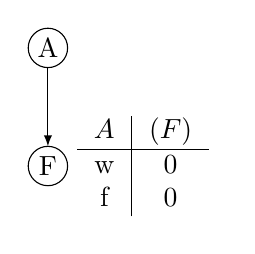
\begin{tikzpicture}[scale=.5]
\draw  (0,0) node{A} ellipse (0.5 and 0.5);
\draw  (0,-3) node{F} ellipse (0.5 and 0.5);
\draw [-latex] (0,-0.5) -- (0,-2.5);
\node [right, align=left] at (0.5,-3) {
\begin{tabular}{c | c}
$A$ & $\PP(F)$\\\hline
w & 0\\
f & 0\\
\end{tabular}
};
\end{tikzpicture}
\end{center}
$\Rightarrow F$ ist nicht erfüllbar
\subsection{Ausweg der NP-Vollständigkeit der exakten Inferenz}
Für speziell strukturierte Netze gibt es einen effizienten Algorithmus. Ferner lässt sich die W'keit durch \emph{Sampling} approximieren. Einfachster Ansatz dann: Beginnend mit dem Startknoten des Netzes werden Ereignisse entsprechend ihrer W'keiten gewürfelt.\\
Dieses Sampling wird $n$-mal wiederholt und es wird ein Mittelwert als Schätzer der W'keit berechnet.
\paragraph{Beispiel}
\begin{center}
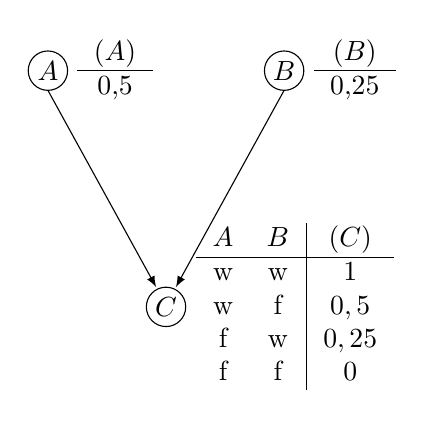
\begin{tikzpicture}[scale=.5]
\draw  (-6,0) node{$A$} ellipse (0.5 and 0.5);
\node [right, align=left] at (-5.5,0) {
\begin{tabular}{c}
$\PP(A)$\\\hline
0,5\\
\end{tabular}
};
\draw  (0,0) node{$B$} ellipse (0.5 and 0.5);
\node [right, align=left] at (0.5,0) {
\begin{tabular}{c}
$\PP(B)$\\\hline
0,25\\
\end{tabular}
};
\draw [-latex] (-6,-0.5) -- (-3.25,-5.5);
\draw [-latex] (0,-0.5) -- (-2.75,-5.5);
\draw (-3,-6) node{$C$} ellipse (0.5 and 0.5);
\node [right=.2, align=left] at (-2.5,-6) {
\begin{tabular}{c c | c}
$A$ & $B$ & $\PP(C)$\\\hline
w & w & $1$\\
w & f & $0,5$\\
f  & w  & $0,25$ \\
f & f& $0$
\end{tabular}
};
\end{tikzpicture}
\end{center}
Sampling Durchlauf:
\begin{enumerate}
\item $A=w$, $B=f$, $C=w$
\item $A=w$, $B=f$, $C=f$
\item $A=f$, $B=f$, $C=f$
\item $A=f$, $B=w$, $C=f$
\item $A=w$, $B=f$, $C=w$
\item $A=f$, $B=f$, $C=f$
\end{enumerate}
Als Schätzer für $\PP(C)$ ergibt sich $\hat{\PP}(C) = \frac{2}{6}=\frac{1}{3}$.\\
Vorteil/Nachteil der Methode:
\begin{itemize}
\item[$+$] Einfach zu implementieren
\item[$-$] Ungeeignet für Netze, in denen Knoten mit sehr geringer Wahrscheinlichkeit vorkommen.
\end{itemize}



